\documentclass{article}
\usepackage[utf8]{inputenc}

\title{Advanced Programming Labwork 6}
\author{Tom HERBRETEAU }
\date{November 2018}

\usepackage{natbib}
\usepackage{graphicx}
\usepackage{pgfplots}
\pgfplotsset{compat=newest}

\begin{document}

\maketitle
Every performance measures are done on ICT4 with eiffel.jpg, without counting the image saving.
\section{Introduction}
We have to implement the map pattern in different kernels. First one binaries the image with a given threshold, the second upper or lower the brightness with a given coefficient, and the last one blend two images with a percentage of each in parameter.
\section{Implementation}
I choose to work with 1D kernel due to results I get in the last labs. For the binari kernel, no bad ugly "if", I divide the current level of gray by the threshold, then I multiply by 255. By the Int cast, gray pixel lower than 127 will be turn into 0 and the higher one will be turn into 255. For the brightness kernel, I just add the brightness coef to the gray pixel. To avoid problem, but WITHOUT IF, I took the max between 0 and result and the min between result and 255, to stay in [0;255], even if the coef is 20, and the initial gray is 246 (246+20 > 255). For the last one, for each pixel, I multiply R, G and B of the first image by the blending percent and R, G and B of the second image by one minus the blending percent and add them to get the output image.
\newline
A way to optimize the two first kernels is to do the grayscale inside the kernel instead of launch it before. 
\section{Result}
Each labs last around 30ms to process. For the example, I choose a threshold equal to 127, a brightness coef equal to -10 and a blend with 50\% of each image.
\newline
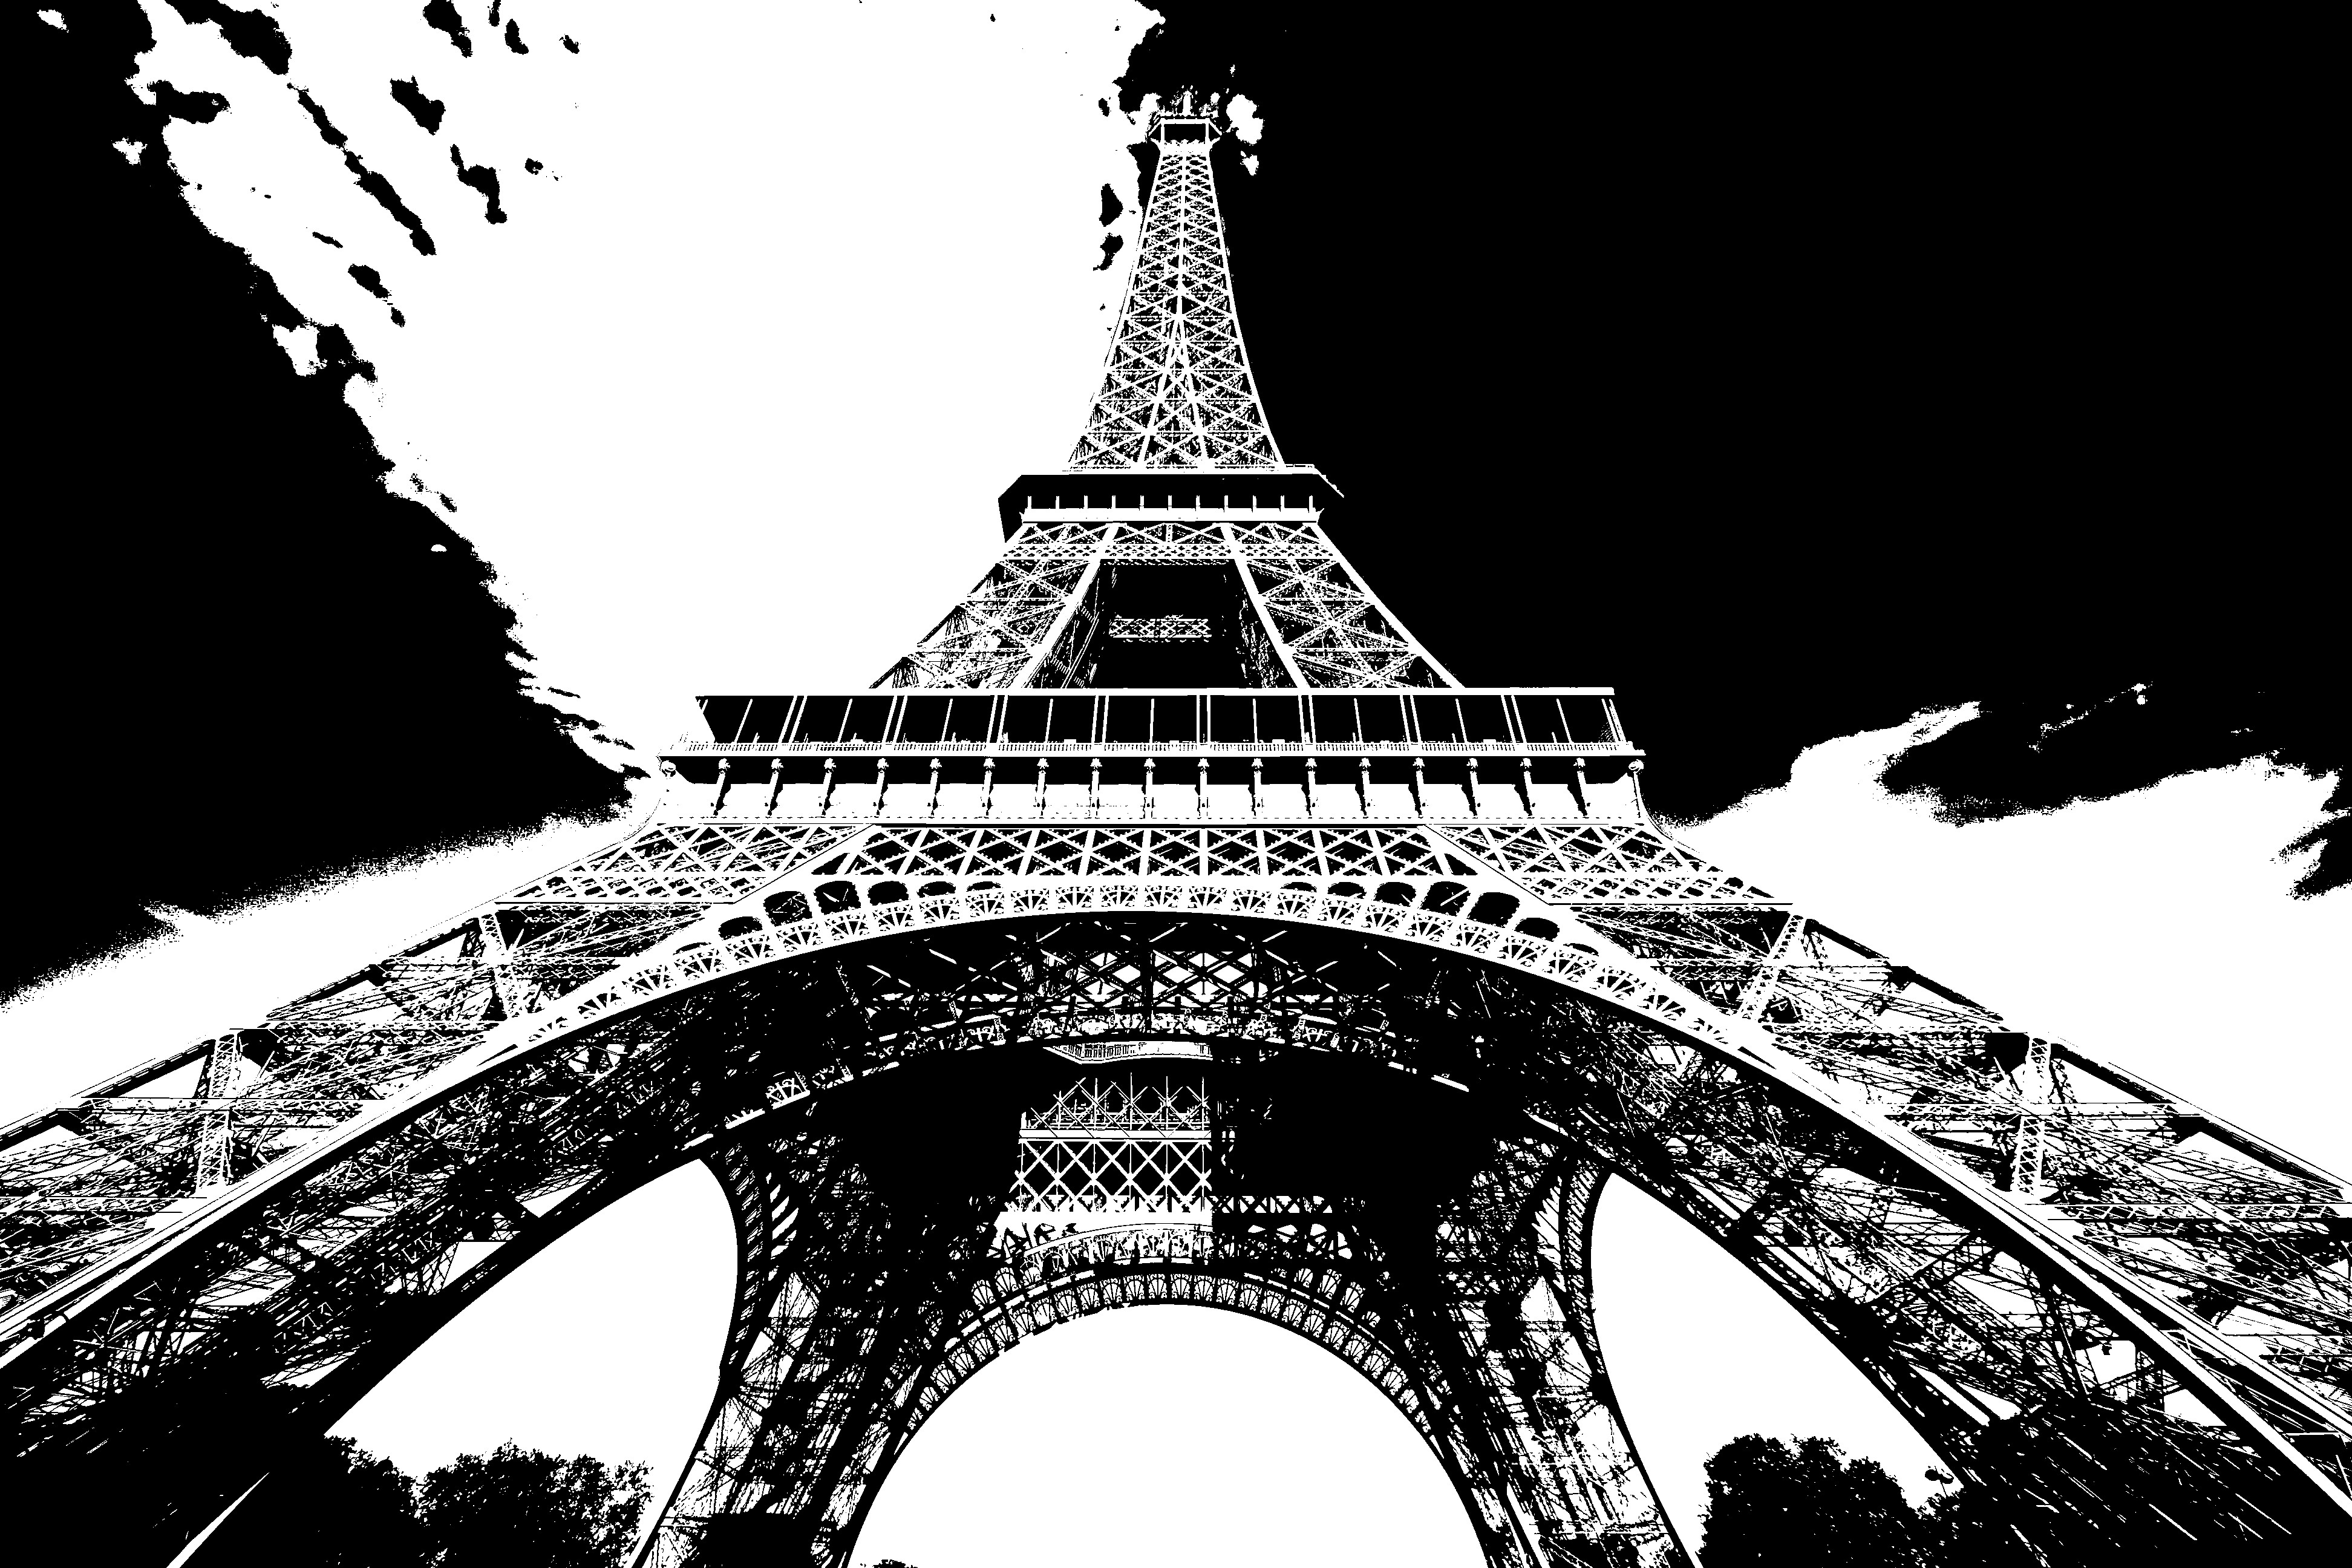
\includegraphics[width=\textwidth]{labwork6-bin-gpu-out.jpg}
\newline
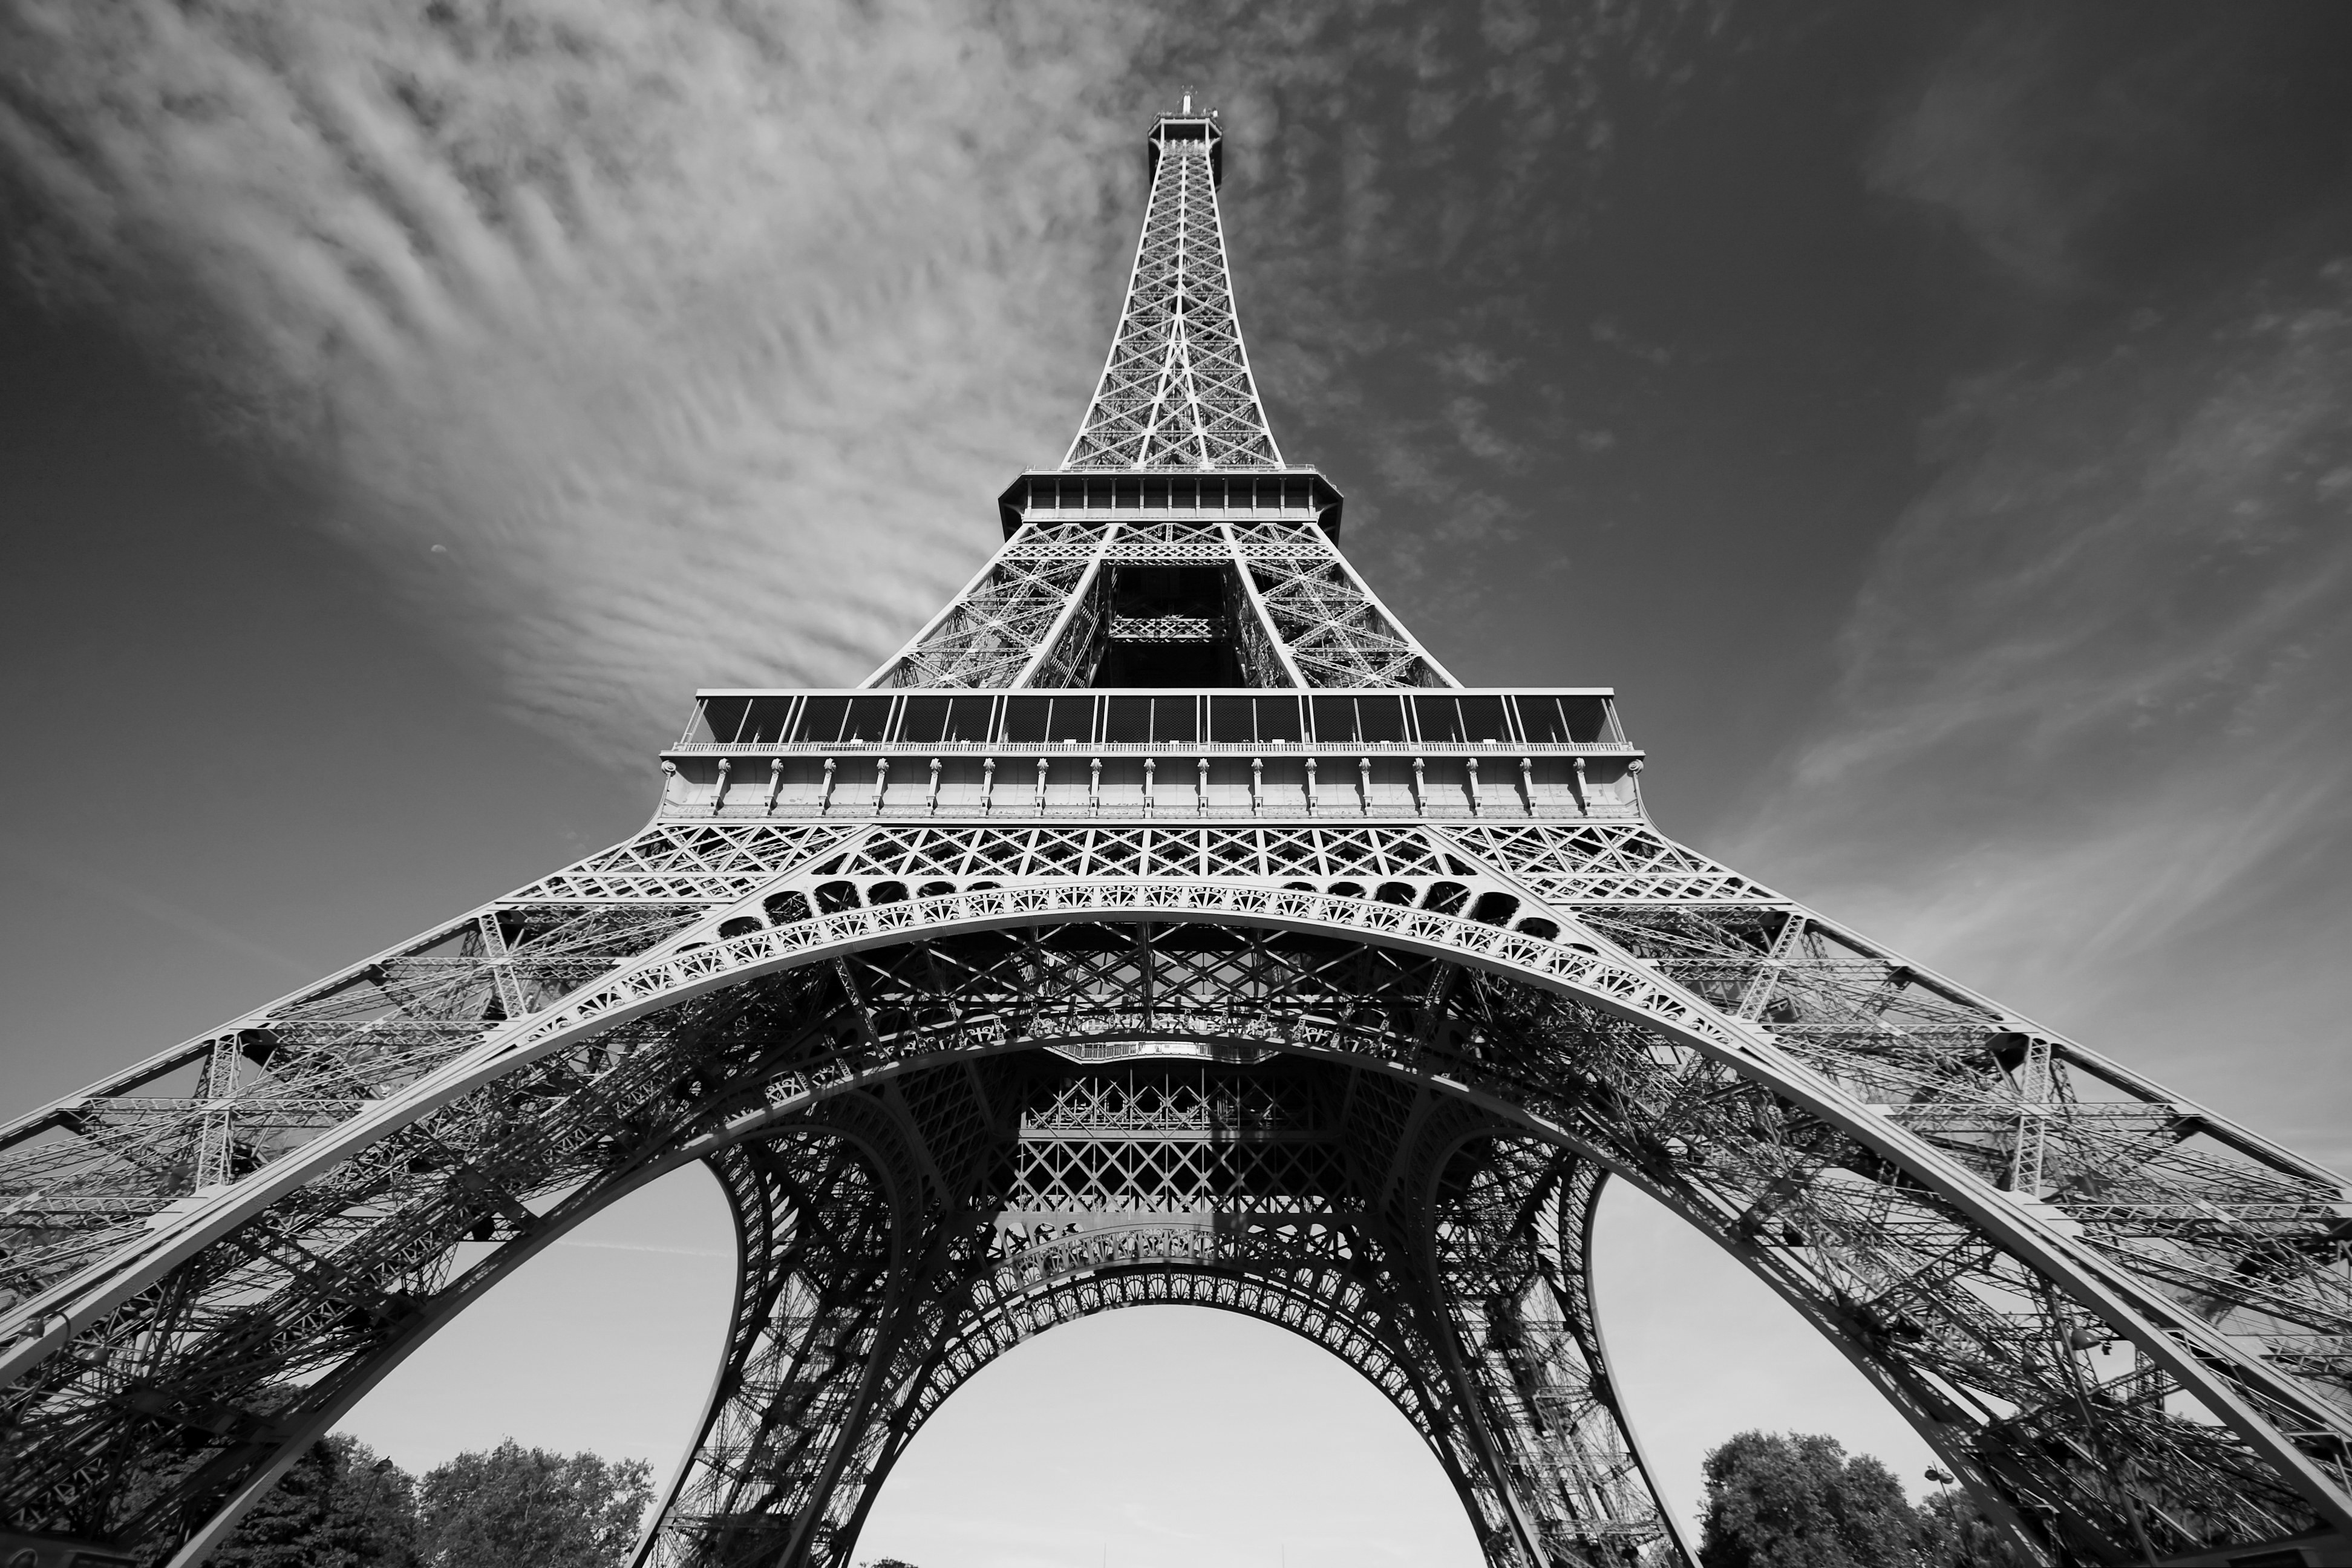
\includegraphics[width=\textwidth]{labwork6-bright-gpu-out.jpg}
\newline
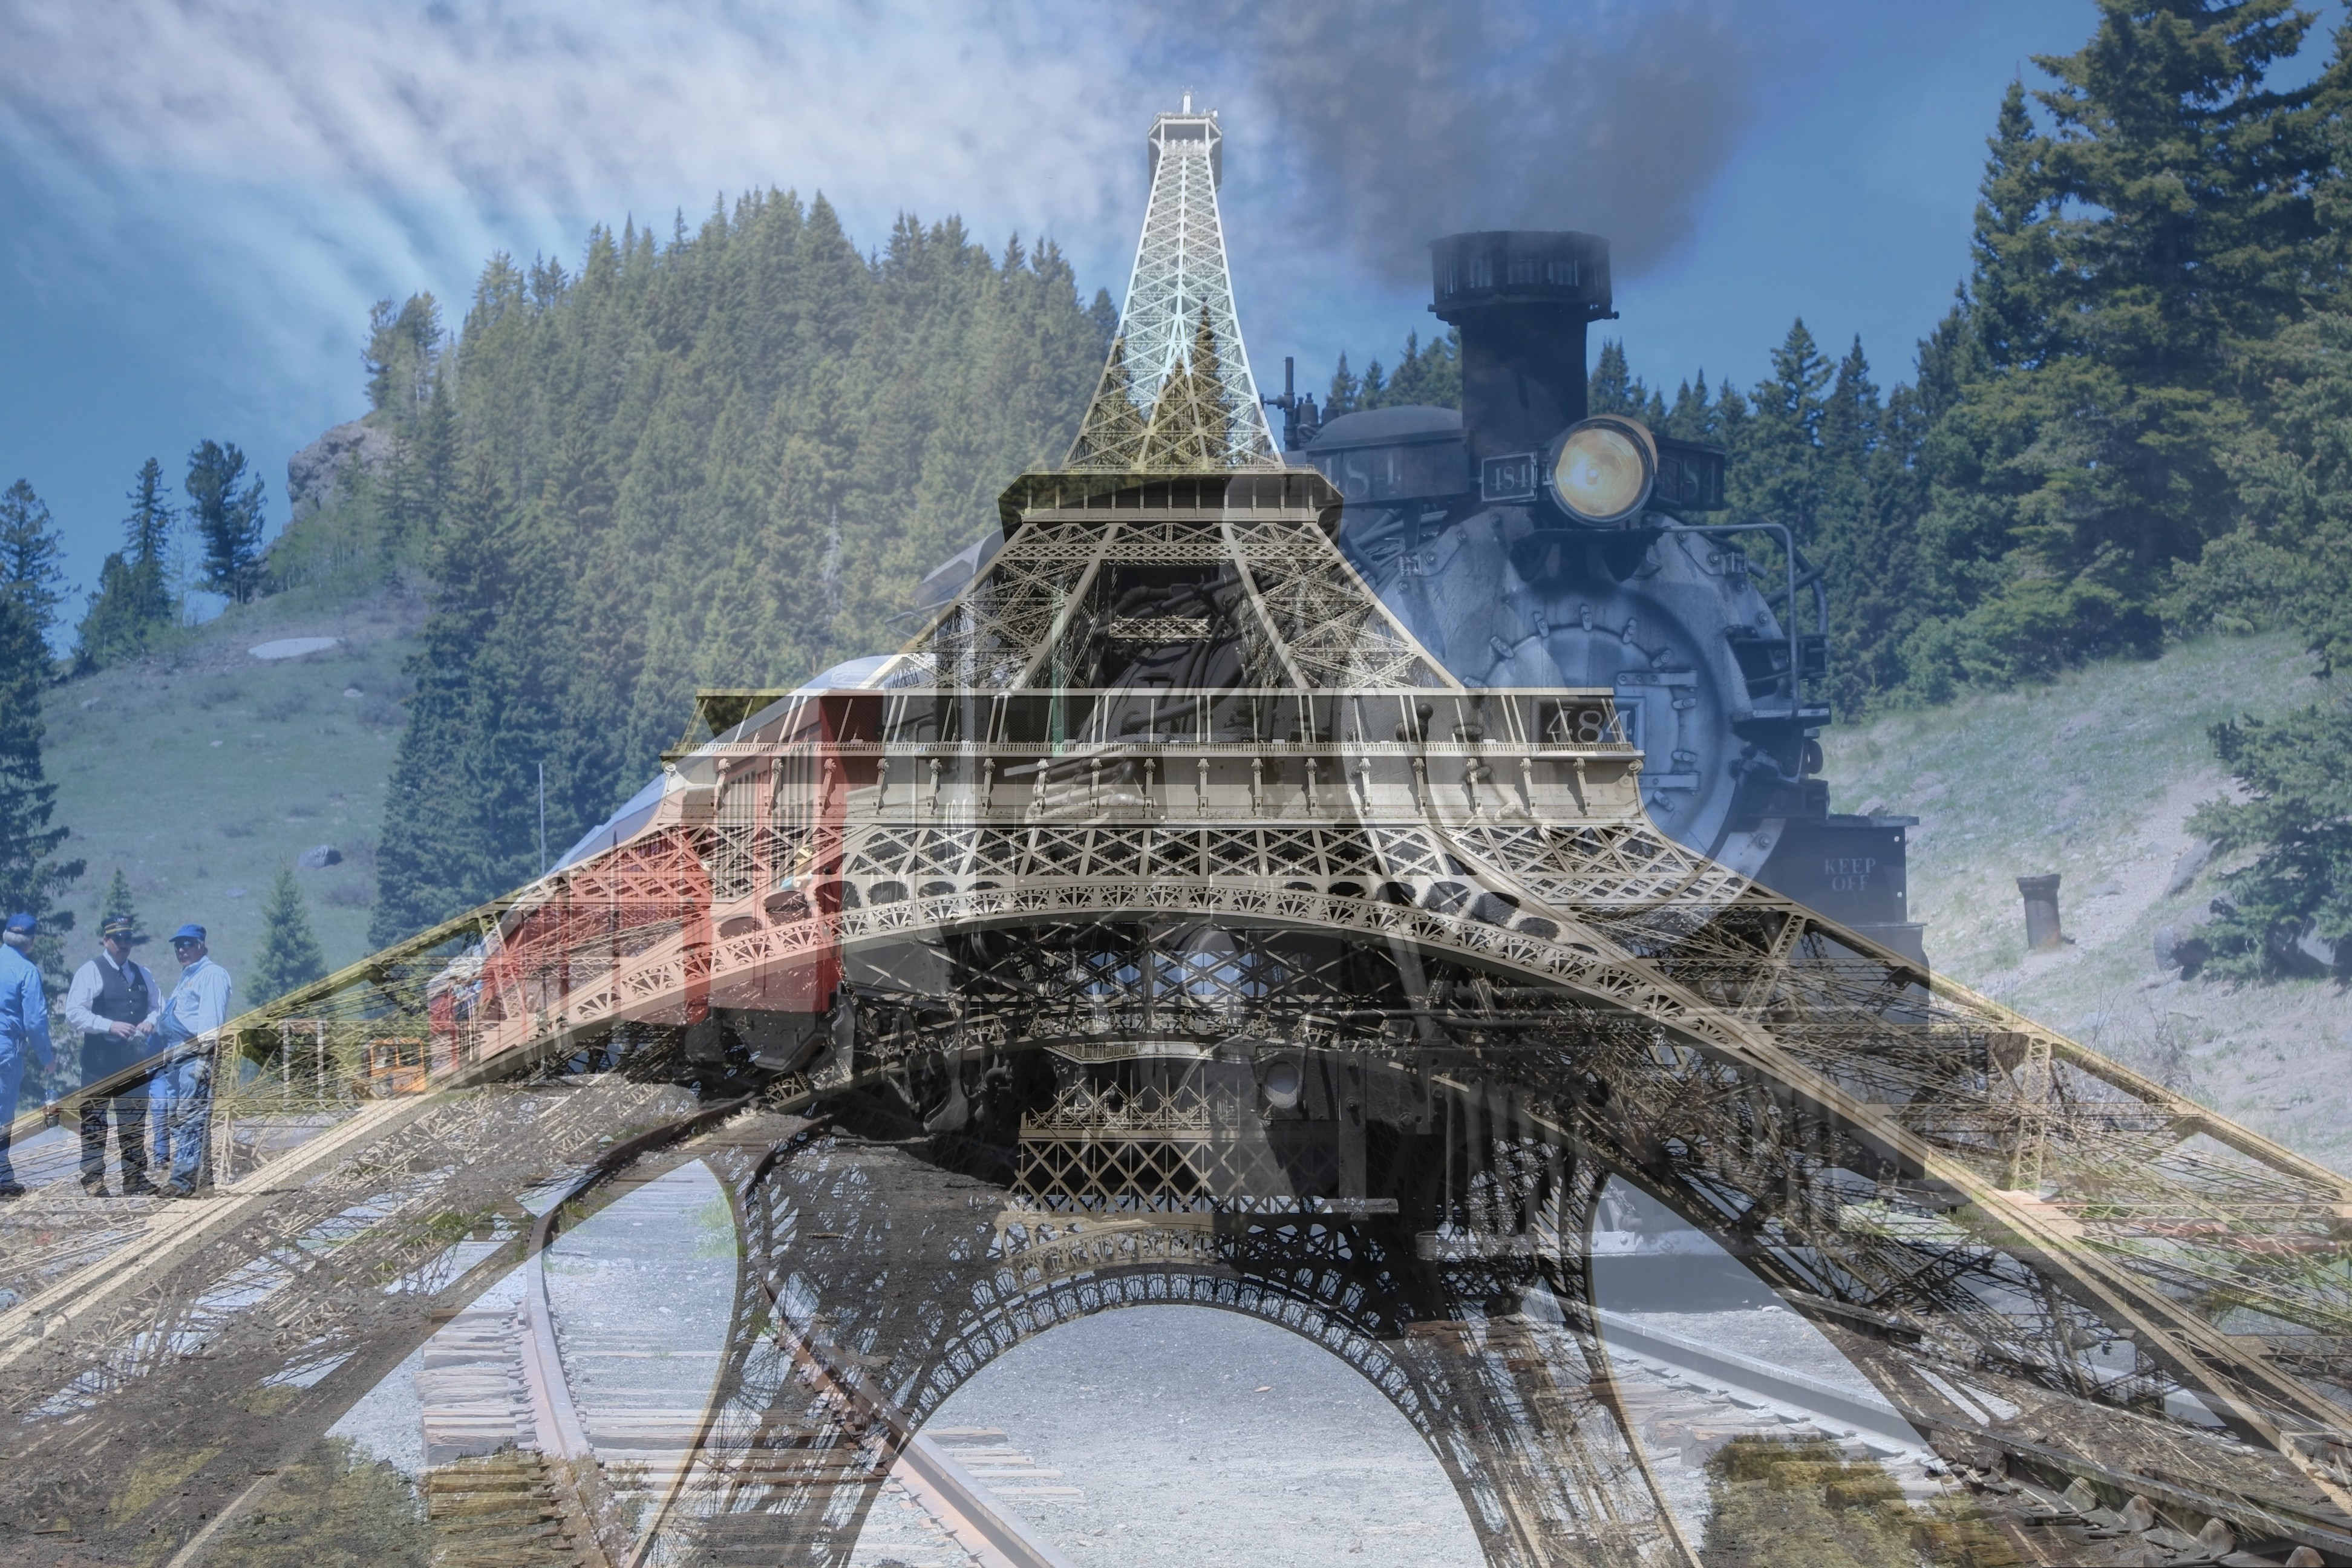
\includegraphics[width=\textwidth]{labwork6-blend-gpu-out.jpg}
\bibliographystyle{plain}
\end{document}
